\section{Ablauf chemischer Reaktionen (Freiwilligkeit)}

\subsection{Enthalpie H / Reaktionsenthalpie (Wärme) $\Delta H_R$}
    Prinzip Energieminimum (Wärmeinhalt eines Systems): Stoff will energiearmen Zustand erreichen!

    $\boxed{\Delta H_R = H_{Produkte} - H_{Edukte}} \quad [H] = \frac{\kilo\joule}{\mol \cdot \kelvin}$

    $\Delta H_R < 0 \Rightarrow$ \textcolor{red}{exotherm, Energieabgabe} $\qquad \Delta H_R > 0 \Rightarrow$ \textcolor{blue}{endotherm, Energieaufnahme}

\subsection{Entropie S (Unordnung) / Reaktionsentropie $\Delta S_R$}
    Prinzip Energiemax: alle Stoffe und Systeme wollen möglichst grosse Entropie

    $\boxed{\Delta S_R = \sum S^0_{Produkte} - \sum S^0_{Edukte}} \qquad \qquad [\Delta S_R] = \frac{\color{red}\joule}{\mol \cdot \kelvin}$

    $S^0$: Molare Standardentropie (1mol des Stoffs bei Std.Bedingungen)

\begin{tabular}{l l}
	$\Delta S_R < 0 \text{  \textbf{Unordnung nimmt ab} z.B. wenn ein Gas zu Flüssigkeit wird}$ &  \\
	$\Delta S_R > 0 \text{  \textbf{Unordnung nimmt zu} z.B. wenn ein Feststoff zu Gas wird}$     &  \\
\end{tabular}

    $\Delta S_R$ abschätzen : Teilchenzahl und Aggregatzustände der Edukte und Produkte beachten

\subsection{Freie Enthalpie $\Delta G$}
    Beschreibt Freiwilligkeit der Reaktion:

    $\boxed{\Delta G = \Delta H - T \cdot \Delta S} \qquad \qquad [\Delta G] = \frac{\kilo\joule}{\mol}$

    $\Delta G < 0:$ Exergon (freiwillige Reaktion) $\qquad \Delta G > 0:$ Endergon(unfreiwillige Reaktion)

    % \begin{itemize}
    %     \item $\Delta G < 0:$ Exergon (freiwillige Reaktion)
    %     \item $\Delta G > 0:$ Endergon(unfreiwillige Reaktion)
    % \end{itemize}

\subsection{Aktivierungsenergie/Reaktionsgeschw. RG/Katalysatoren}\label{Reaktionsgeschw}
\begin{minipage}{0.32\linewidth}
    % \vspace*{0pt}
    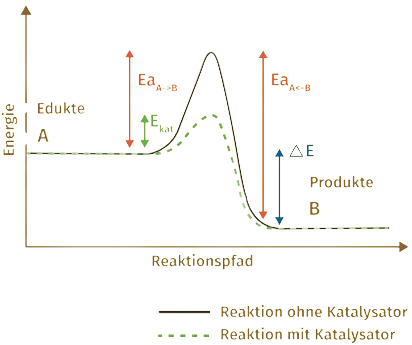
\includegraphics[width=\linewidth]{pictures/Katalysator_1.png}
\end{minipage}
\hfill
\begin{minipage}{0.65\linewidth}
    \begin{itemize}
        \item RGT-Regel: $\Delta$T = $+10\degree C$ $\rightarrow$ RG $\cdot$ 2
        \item Katalysator = Stoff nimmt an Reaktion teil, wird nicht verbraucht 
        \item Beschleunigt Reaktion: $E_{AKat} \ll E_{ANorm}$
        \item $\Delta$ G sowie $\Delta H_R$ bleiben gleich
        \item Selektiv (wirkt nicht mit allen Stoffen)
    \end{itemize}
\end{minipage}
